\chapter{ Констукторский раздел}
\label{cha:design}
    В данном разделе описаны разработанные алгоритмы, а также используемые классы.
    \section{Разработка алгоритмов решения поставленной задачи}
    \subsection{Общий алгоритм}
    \par Общий алгоритм задачи подразумевает, что основной функционал программы выполняется в бесконечном цикле. 
    \begin{figure}[h!]
            \centering
            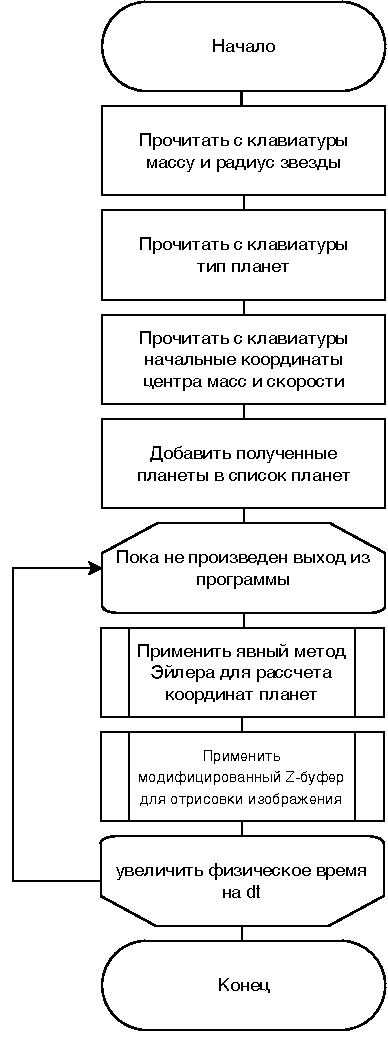
\includegraphics[scale=0.8]{inc/All_alg.pdf}
            \caption{Схема Общего алгоритма}
            \label{schema:All_alg}
        \end{figure}\clearpage
    \subsection{Модифицированный алгоритм $Z$-буфера}
    \par Модификация алгоритма $Z$-буфера заключается в том, что в буфере будут храниться координаты $z$ только для центров планет.
    \par Так как планеты не должны пересекаться, по координатам их центра можно однозначно определить их расположение относительно экранной плоскости. Также предлагается отрисовывать только те точки сетки сферы, глубина которых не меньше глубины центра сферы.
    \par На рисунке \ref{schema:Z_alg_1} представлена схема алгоритма модифицированного Z-буфера.
    \begin{figure}[h!]
            \centering
            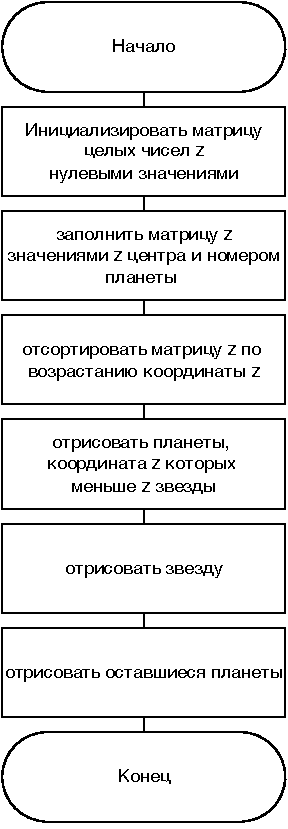
\includegraphics[scale=0.8]{inc/Z.pdf}
            \caption{Схема модифицированного Z-буфера}
            \label{schema:Z_alg_1}
    \end{figure}\clearpage
    \subsection{Алгоритм построения полигональной сетки}
    \par На рисунке \ref{schema:Pol_alg_1} представлена схема алгоритма построения полигональной сетки.
    \begin{figure}[h!]
            \centering
            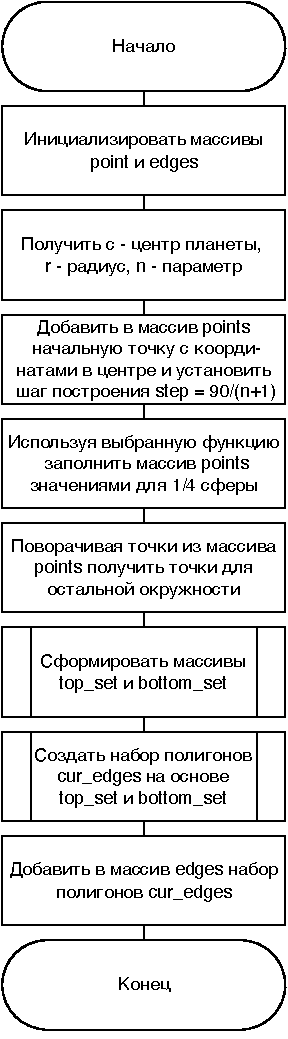
\includegraphics[scale=0.8]{inc/Pol_al.pdf}
            \caption{Схема алгоритма полигональной сетки}
            \label{schema:Pol_alg_1}
    \end{figure}\clearpage
    \subsection{Алгоритм простой закраски}
    \par На рисунке \ref{schema:P_zak} представлена схема алгоритма простой закраски.
    \begin{figure}[h!]
            \centering
            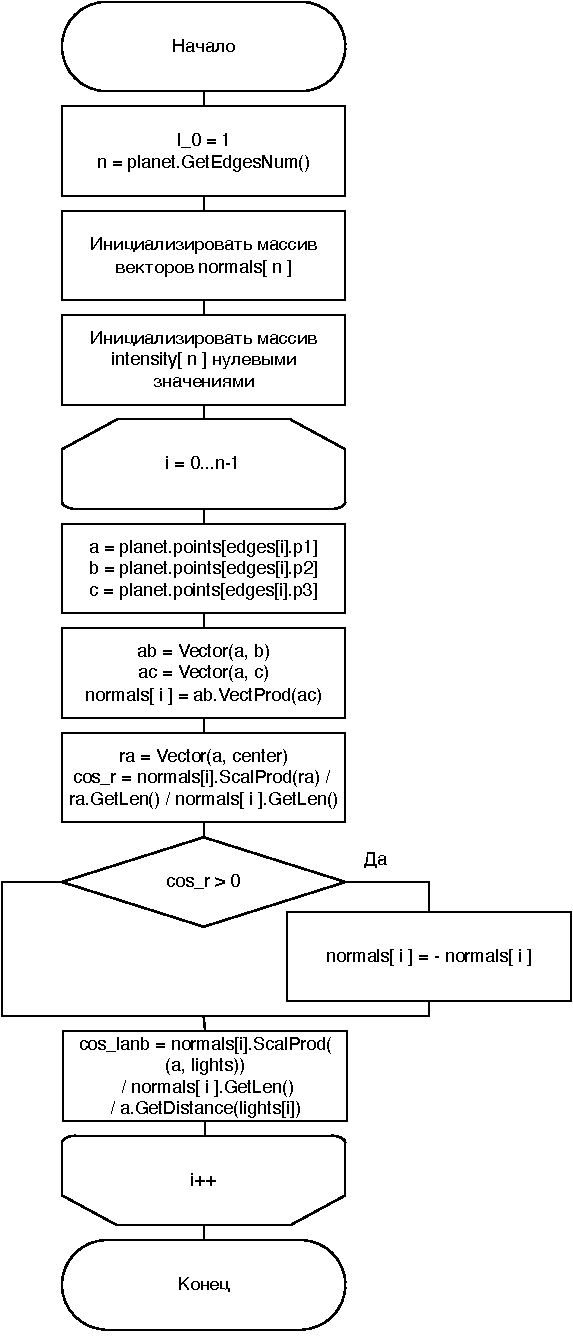
\includegraphics[scale=0.8]{inc/P_zak.pdf}
            \caption{Схема алгоритма простой закраски}
            \label{schema:P_zak}
    \end{figure}\clearpage
    \subsection{Используемые типы и структуры данных}
    \par В таблице \ref{table:StructTypes} представлены типы и структуры данных, которые будут реализованы для разрабатываемого ПО.

    \begin{table}[]
        \caption{Используемые типы и структуры данных}
        \centering
\begin{tabular}{|l|l|}
\hline
Сущность & Структура                                                                                                                                         \\ \hline
Точка с координатами X, Y, Z & Структура Point \\ \hline
\begin{tabular}[c]{@{}l@{}}Вектор с начальной  и конечной \\ точками\end{tabular} & Структура Vector \\ \hline
Полигон с индексом трех точек & Структура Edge \\ \hline
\begin{tabular}[c]{@{}l@{}}Объект с координатами центра, радиусом, \\ типом объекта, параметром узлов сетки, \\ массивом точек, массивом полигонов\end{tabular} & Структура Object \\ \hline
\begin{tabular}[c]{@{}l@{}}Планета со всеми параметрами объекта, \\ цветом поверхности и списком \\ интенсивности граней\end{tabular} & Структура Planet \\ \hline
\begin{tabular}[c]{@{}l@{}}Звезда со всеми параметрами объекта \\ и списком координат источников света\end{tabular} & Структура Star \\ \hline
\begin{tabular}[c]{@{}l@{}}Сцена со звездой, массивом планет\\ и с таймером для покадровой анимации\end{tabular} & Структура MyGraphicsView \\ \hline

\end{tabular}
        \label{table:StructTypes}
    \end{table}
    \section{Выводы из конструкторской части}
    \par В данном разделе были описаны схемы реализуемых алгоритмов, определены используемые сущности и структуры данных.
\newpage